\documentclass[10pt]{beamer}
\usetheme[
%%% options passed to the outer theme
%    hidetitle,           % hide the (short) title in the sidebar
%    hideauthor,          % hide the (short) author in the sidebar
%    hideinstitute,       % hide the (short) institute in the bottom of the sidebar
%    shownavsym,          % show the navigation symbols
%    width=2cm,           % width of the sidebar (default is 2 cm)
%    hideothersubsections,% hide all subsections but the subsections in the current section
%    hideallsubsections,  % hide all subsections
    left               % right of left position of sidebar (default is right)
%%% options passed to the color theme
%    lightheaderbg,       % use a light header background
  ]{AAUsidebar}

% If you want to change the colors of the various elements in the theme, edit and uncomment the following lines
% Change the bar and sidebar colors:
%\setbeamercolor{AAUsidebar}{fg=red!20,bg=red}
%\setbeamercolor{sidebar}{bg=red!20}
% Change the color of the structural elements:
%\setbeamercolor{structure}{fg=red}
% Change the frame title text color:
%\setbeamercolor{frametitle}{fg=blue}
% Change the normal text color background:
%\setbeamercolor{normal text}{bg=gray!10}
% ... and you can of course change a lot more - see the beamer user manual.

\usepackage[utf8]{inputenc}
\usepackage[english]{babel}
\usepackage[T1]{fontenc}
% Or whatever. Note that the encoding and the font should match. If T1
% does not look nice, try deleting the line with the fontenc.
\usepackage{helvet}

% colored hyperlinks
\newcommand{\chref}[2]{%
  \href{#1}{{\usebeamercolor[bg]{AAUsidebar}#2}}%
}

\title[Compilateur Kawa]% optional, use only with long paper titles
{Compilateur Kawa}

\subtitle{Projet annuel}  % could also be a conference name

\date{Lundi 19 Janvier 2015}

\author[ADJIBI Nasser, PETRE Alexandre, TASSERIE Majid, BLOT Pierre-Luc, BERKANE Kheireddine, IDRISSOU Hamzath, AHOUATE Abdellatif] % optional, use only with lots of authors
{
  ADJIBI Nasser, PETRE Alexandre, TASSERIE Majid, BLOT Pierre-Luc, BERKANE Kheireddine, IDRISSOU Hamzath, AHOUATE Abdellatif
}
% - Give the names in the same order as they appear in the paper.
% - Use the \inst{?} command only if the authors have different
%   affiliation. See the beamer manual for an example

\institute[
%  {\includegraphics[scale=0.2]{aau_segl}}\\ %insert a company, department or university logo
  Dept.\ informatique\\
  Université de Rouen\\
  2014-2015
] % optional - is placed in the bottom of the sidebar on every slide
{% is placed on the title page
  Département informatique\\
  Université de Rouen\\
  2014-2015
  %there must be an empty line above this line - otherwise some unwanted space is added between the university and the country (I do not know why;( )
}


% specify a logo on the titlepage (you can specify additional logos an include them in 
% institute command below
\pgfdeclareimage[height=1.5cm]{titlepagelogo}{AAUgraphics/logo_univ} % placed on the title page
%\pgfdeclareimage[height=1.5cm]{titlepagelogo2}{graphics/aau_logo_new} % placed on the title page
\titlegraphic{% is placed on the bottom of the title page
  \pgfuseimage{titlepagelogo}
%  \hspace{1cm}\pgfuseimage{titlepagelogo2}
}


\begin{document}
% the titlepage
{\aauwavesbg%
\begin{frame}[plain,noframenumbering] % the plain option removes the sidebar and header from the title page
  \titlepage
\end{frame}}
%%%%%%%%%%%%%%%%

% TOC
\begin{frame}{Sommaire}{}
\tableofcontents
\end{frame}
%%%%%%%%%%%%%%%%
\section{Introduction}
% motivation for creating this theme
  \subsection{Présentation de l'équipe}
    \begin{frame}{Introduction}{Présentation de l'équipe}
      \begin{block}{Présentation de l'équipe}
        \begin{figure}[!h]
          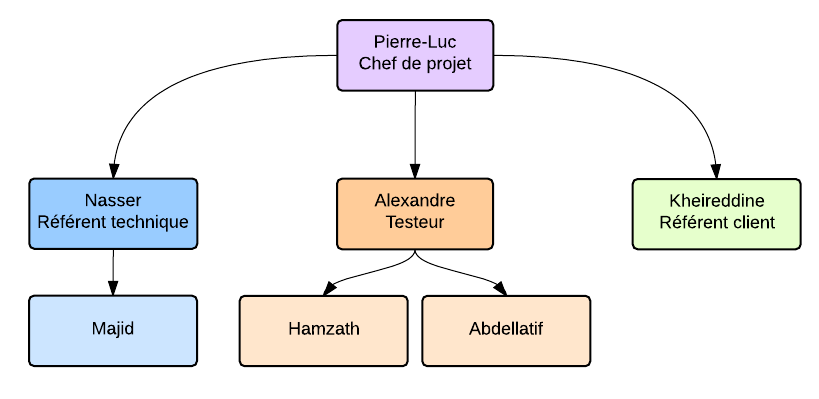
\includegraphics[width=7cm]{../pdd/fig/organigramme.png}
          \caption{Organisation de l'équipe.}
          \label{organisaiton_de_l_equipe}
        \end{figure}      
      \end{block}
    \end{frame}
%%%%%%%%%%%%%%%%

\section{Analyse des besoins du client}
    \begin{frame}{Analyse des besoins du client}
      \begin{itemize}
        \item<1-> Langage imposé {\tt Kawa}
        \item<2-> Technologie imposée {\tt LLVM}
        \item<3-> Pourquoi kawa ?
          \begin{itemize}
            \item<4-> Langage qui est similaire à java.
            \item<5-> Bénéficier des fonctionnalités d'un langage de haut niveau ainsi que des performances bas niveau.
            \item<6-> Compiler kawa en code natif sans passer par une machine virtuelle.
          \end{itemize}
        
      \end{itemize}
    \end{frame}

  \subsection{Notions supportées par les modes de compilation}
    \begin{frame}{Analyse des besoins du client}{Notions supportées par les modes de compilation}
      \begin{block}{Notions supportées par les modes de compilation}
        \begin{itemize}
          \item<1-> Classe, classe abstraite et interface.
          \item<2-> Héritage
          \item<3-> Polymorphisme
          \item<4-> Contrôle de types
        \end{itemize}
      \end{block}
    \end{frame}
    %%%%
    \begin{frame}{Analyse des besoins du client}{Notions supportées par les modes de compilation}
      \begin{block}{Modes de compilation}
        \begin{itemize}
          \item<1-> Compilation d'une application en mode monolithique
          \item<2-> Compilation d'une application en mode partagé.
          \item<3-> Compilation d'une bibliothèque partagée.
        \end{itemize}
      \end{block}
    \end{frame}
%%%%%%%%%%%%%%%%
\section{Plan de développement}
  \subsection{Diagramme de Gantt}
    \begin{frame}{Plan de développement}{Diagramme de Gantt}
      \begin{figure}[!h]
          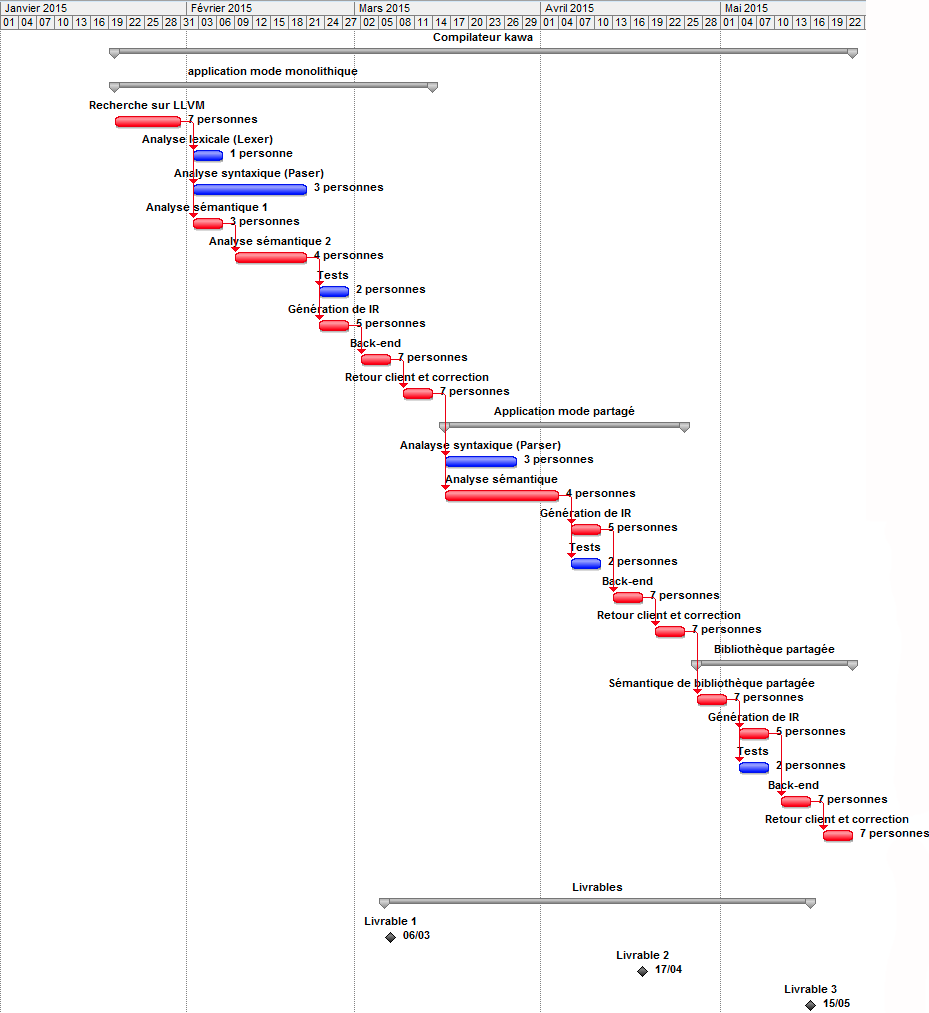
\includegraphics[width=7cm]{../pdd/fig/decoupage_cycles.png}
          \caption{Decoupage général en cycles.}
          \label{decoupage_cycles}
        \end{figure}
    \end{frame}
  \subsection{Stratégie de livraison en itérations}
    \begin{frame}{Plan de développement}{Stratégie de livraison en itérations}
      \begin{block}{Itération 1: Application en mode monolitique}
        
           \begin{itemize}
             \item<1-> Livraison le 06/03/2015
             \item<2-> Contenu: 
              \begin{itemize}
                \item<3-> Héritage.
                \item<4-> Polymorphisme.
              \end{itemize}
           \end{itemize}
        
      \end{block}
    \end{frame}
    %%%%
    \begin{frame}{Plan de développement}{Stratégie de livraison en itérations}
      \begin{block}{Itération 2: Application en mode partagé}
       
           \begin{itemize}
             \item<1-> Livraison le 17/04/2015
             \item<2-> Contenu:
              \begin{itemize}
                \item<3-> Héritage.
                \item<4-> Polymorphisme.
                \item<5-> Contrôle de typage.
              \end{itemize}
           \end{itemize}
        
      \end{block}
    \end{frame}
    %%%%
    \begin{frame}{Plan de développement}{Stratégie de livraison en itérations}
      \begin{block}{Itération 3: Livraison finale}
       
           \begin{itemize}
             \item<1-> Livraison le 15/05/2015
             \item<2-> Contenu: 
              \begin{itemize}
                \item<3-> Compilation en mode monolitique.
                \item<4-> Compilation d'application en mode partagé.
                \item<5-> Compilation de bibliothèque partagée.
              \end{itemize}
           \end{itemize}
        
      \end{block}
    \end{frame}
%%%%%%%%%%%%%%%%
\section{Analyse des risques}
     \begin{frame}{Analyse des risques}{Introduction}
        Introduction ADR....
     \end{frame}
   %%%%
   \subsection{Risques}
     \begin{frame}{Analyse des risques}{Incapacité du client/d'un membre du groupe}
        \begin{block}{Incapacité du client/d'un membre du groupe}
          \begin{itemize}
            \item Criticité: critique / préoccupant
            \item Probabilité: faible / moyenne
          \end{itemize}
        \end{block}
      \end{frame}
      %%%%
      \begin{frame}{Analyse des risques}{Projet insatisfaisant/incomplet}
        \begin{block}{Projet insatisfaisant/incomplet}
          \begin{itemize}
            \item Criticité: critique
            \item Probabilité: faible
          \end{itemize}
        \end{block}
      \end{frame}
      %%%%
      \begin{frame}{Analyse des risques}{Retard dans le projet}
        \begin{block}{Retard dans le projet}
          \begin{itemize}
            \item Criticité: important
            \item Probabilité: forte / moyenne
          \end{itemize}
        \end{block}
      \end{frame}
      %%%%
      \begin{frame}{Analyse des risques}{Abandon d'un membre de l'équipe}
        \begin{block}{Abandon d'un membre de l'équipe}
          \begin{itemize}
            \item Criticité: important
            \item Probabilité: moyenne
          \end{itemize}
        \end{block}
      \end{frame}
  %%%%%%%%%%%%%%%
\section{Cahier de recettes}
     \begin{frame}{Cahier de recettes}{Introduction}
        Introduction ....
     \end{frame}
   %%%%
   \subsection{Mise en place}
      \begin{frame}{Cahier de recettes}{Mise en place}
        \begin{block}{Mise en place}
          Lancement d'une phase de test après chaque fonctionnalité implantée:
          \begin{itemize}
            \item<1-> Mise en place de tests spécifiques
            \item<2-> Vérification du bon foncitonnement
            \item<3-> Possibilité de mise en place de tests de non-régression
            \item<4-> Retour développeur
          \end{itemize}
        \end{block}
      \end{frame}
      %%%%
   \subsection{Spécificité des tests}
      \begin{frame}{Cahier de recettes}{Spécificité des tests}
        \begin{block}{Test Unitaire}
          \begin{itemize}
            \item<1-> Objectif: Vérifier la validité d'un module de code.
            \begin{itemize}
              \item<2-> Fonctionnalité
              \item<3-> Exigence précise
            \end{itemize}
          \end{itemize}
        \end{block}
      \end{frame}
      %%%%
      \begin{frame}{Cahier de recettes}{Spécificité des tests}
        \begin{block}{Test d'intégration}
          \begin{itemize}
            \item<1-> Objectif: Vérifier la validité d'un ensemble de fonctionnalités afin d'en faire uin livrable.
          \end{itemize}
        \end{block}
      \end{frame}
      %%%%
      \begin{frame}{Cahier de recettes}{Spécificité des tests}
        \begin{block}{Test de non-régression}
          \begin{itemize}
            \item<1-> Objectif: Vérifier que l'ajout de fonctionnalités n'a pas eu de répercussion sur l'existant.
            \item<2-> Pas toujours nécessaire.
          \end{itemize}
        \end{block}
      \end{frame}

    \subsection{Approche d'écriture des tests}
      \begin{frame}{Cahier de recettes}{Approche d'écriture des tests}
        \begin{block}{Réutilisation}
          \begin{itemize}
            \item<1-> Écriture automatisée
            \item<2-> Écriture du code pour lancer tests
            \item<3-> Vérification des résultats
          \end{itemize}
        \end{block}
      \end{frame}
      \begin{frame}{Cahier de recettes}{Approche d'écriture des tests}
        \begin{block}{Objectifs}
          \begin{itemize}
            \item<1-> Augmenter la complexité des tests facilement
            \item<2-> Éviter la redondance dans l'écriture des tests
            \item<3-> Valider avec une plus grande certitude le bon déroulement des fonctions.
          \end{itemize}
        \end{block}
      \end{frame}

      \subsection{Objectifs des tests}
      \begin{frame}{Cahier de recettes}{Objectifs des tests}
        \begin{block}{Objectifs des tests}
          \begin{itemize}
            \item<1-> Vérifier que chaque fonctionnalités réalise sa tâche correctement.
            \item<2-> Valider des modules.
            \item<3-> Réaliser une large couverture de code.
          \end{itemize}
        \end{block}
      \end{frame}  
  %%%%%%%%%%%%%%%
\section{Solutions aux exigences de client}
     \begin{frame}{Solutions aux exigences de client}{}
        \begin{itemize}
          \item<1-> Analyse lexicale couplée avec l'analyse syntaxique
          \item<2-> Génération d’un arbre syntaxique abstrait couplée avec une analyse sémantique.
          \item<3-> Génération du code intermédiaire.
          \item<4-> Compilation du code intermédiaire en objet machine.
        \end{itemize}
     \end{frame}
   %%%%
   \subsection{Schématisation de la compilation}
      \begin{frame}{Solutions aux exigences de client}{Schématisation de la compilation}
        \begin{block}{Schématisation de la compilation}
          \begin{figure}[!h]
            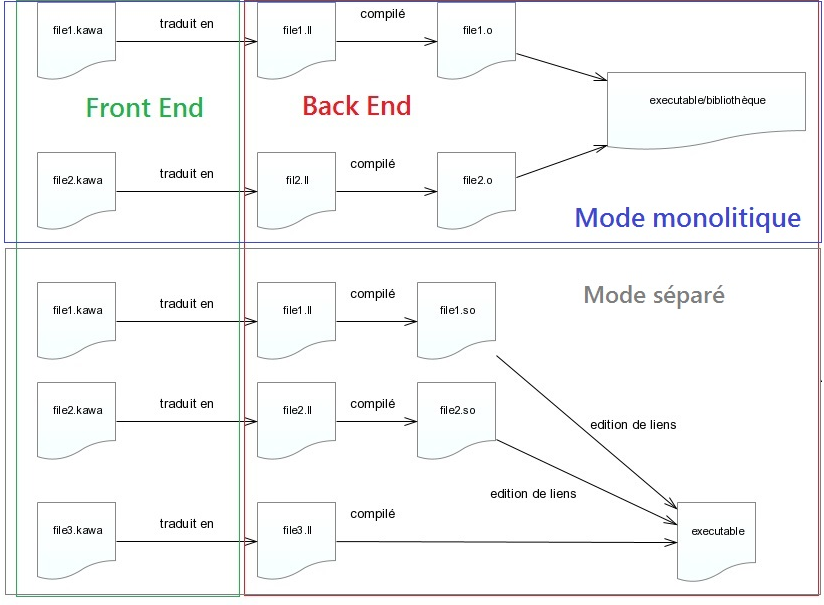
\includegraphics[width=8cm]{../res/presentation/fig2.png}
            \caption{Processus de compilation}
            \label{processus_de_compilation}
          \end{figure}
        \end{block}
      \end{frame}
    %%%%
   \subsection{Outils de réalisation}
      \begin{frame}{Solutions aux exigences de client}{Outils de réalisation Front End}
        \begin{block}{Outils de réalisation Front End}
          \begin{itemize}
            \item<1-> Langage de programmation: C++
            \begin{itemize}
              \item<2-> Contrainte imposée par le client motivé par la disponibilité d'une API LLVM permettant la production du code intermédiaire LLVM.
            \end{itemize}
            \item<3-> Langage Cible: code IR LLVM
            \begin{itemize}
              \item<4-> Le code IR LLVM est un langage à part entière capable de réaliser les exigences du client. 
            \end{itemize}
          \end{itemize}
        \end{block}
      \end{frame}
    
      \begin{frame}{Solutions aux exigences de client}{Outils de réalisation Back End}
        \begin{block}{Outils de réalisation Back End}
          \begin{itemize}
            \item<1-> Outils de compilation de code intermédiaire
            \begin{itemize}
              \item<2-> opt: Optimisation de code LLVM
              \item<3-> llc: Compilateur de code IR
              \item<4-> lld: Éditeur de lien
              \item<5-> clang: Compilateur compatible code IR.
            \end{itemize}
            
          \end{itemize}
        \end{block}
      \end{frame}
       %%%%
    \subsection{Extension du document d'architecture}
      \begin{frame}{Solutions aux exigences de client}{Extension du document d'architecture}
        \begin{block}{Extension du document d'architecture}
          \begin{itemize}
            \item<1-> Des détails de la réalisation seront à résoudre lors du processus de développement.
            \item<2-> Impossible de fournir une architecture garantissant à 100\% la réalisation du projet. 
            \item<3-> Les découvertes faites seront rajoutées au document d’architecture logiciel.
          \end{itemize}
        \end{block}
      \end{frame}
  
  %%%%%%%%%%%%%%%
\section{Conclusion}
\begin{frame}{Conclusion}
  Projet LLVM : Compilateur Kawa
  \begin{center}
    \insertauthor
  \end{center}
\end{frame}
%%%%%%%%%%%%%%%%

{\aauwavesbg
\begin{frame}[plain,noframenumbering]
  \finalpage{Merci pour votre attention !\\
  Avez-vous des questions ?
  }
\end{frame}}
%%%%%%%%%%%%%%%%

\end{document}
